%%%%%%%%%%%%%%%%%%%%%%%%%%%%%%%%%%%%%%%%%
% NIWeek 2014 Poster by T. Reveyrand
% www.microwave.fr
% http://www.microwave.fr/LaTeX.html
% ---------------------------------------
%
% Original template created by:
% Brian Amberg (baposter@brian-amberg.de)
%
% This template has been downloaded from:
% http://www.LaTeXTemplates.com
%
% License:
% CC BY-NC-SA 3.0 (http://creativecommons.org/licenses/by-nc-sa/3.0/)
%
%%%%%%%%%%%%%%%%%%%%%%%%%%%%%%%%%%%%%%%%%

%----------------------------------------------------------------------------------------
%	PACKAGES AND OTHER DOCUMENT CONFIGURATIONS
%----------------------------------------------------------------------------------------

\documentclass[a0paper,portrait]{baposter}

\usepackage[font=small,labelfont=bf]{caption} % Required for specifying captions to tables and figures
\usepackage{booktabs} % Horizontal rules in tables
\usepackage{relsize} % Used for making text smaller in some places

\usepackage{amsmath,amsfonts,amssymb,amsthm} % Math packages
\usepackage{eqparbox}

%============
\usepackage[utf8]{inputenc}
\usepackage{xcolor}
\usepackage{graphicx}
\usepackage{MnSymbol}
\usepackage{stmaryrd}
\usepackage{colortbl}
\usepackage{caption}
\usepackage{comment}
\usepackage[utf8]{inputenc}
\usepackage{pdfpages}
\usepackage{listings}
\usepackage{color}
\usepackage{booktabs}
\usepackage{soul}
\usepackage[normalem]{ulem}
\usepackage{float}
\usepackage{color}
\usepackage{tcolorbox}
\usepackage{lipsum}

\newcommand{\Ep}{\mathbb{E}}
\newcommand{\Real}{\mathcal{R}}
\newcommand{\Rating}{\mathbf{X}}
\newcommand{\Loss}{\mathcal{L}}

\usepackage{pgf}
%\usepackage{etex}
\usepackage{tikz,pgfplots}
\usetikzlibrary{matrix,arrows,decorations.pathmorphing}
%\usetikzlibrary{tikzmark}

%============
\usepackage{textcomp}

\graphicspath{{figures/}} % Directory in which figures are stored

 \definecolor{bordercol}{RGB}{40,40,40} % Border color of content boxes
 \definecolor{headercol1}{RGB}{186,215,230} % Background color for the header in the content boxes (left side)
 \definecolor{headercol2}{RGB}{120,120,120} % Background color for the header in the content boxes (right side)
 \definecolor{headerfontcol}{RGB}{0,0,0} % Text color for the header text in the content boxes
 \definecolor{boxcolor}{RGB}{255,255,255} % {210,235,250} Background color for the content in the content boxes

\begin{document}

\background{ % Set the background to an image (background.pdf)
\begin{tikzpicture}[remember picture,overlay]
\draw (current page.north west)+(-2em,2em) node[anchor=north west]
{
\includegraphics[height=1.1\textheight]{background}};
\end{tikzpicture}
}

\begin{poster}{
grid=false,
borderColor=bordercol, % Border color of content boxes
headerColorOne=headercol1, % Background color for the header in the content boxes (left side)
headerColorTwo=headercol2, % Background color for the header in the content boxes (right side)
headerFontColor=headerfontcol, % Text color for the header text in the content boxes
boxColorOne=boxcolor, % Background color for the content in the content boxes
headershape=roundedright, % Specify the rounded corner in the content box headers
headerfont=\Large\sf\bf, % Font modifiers for the text in the content box headers
textborder=rectangle,
background=user,
headerborder=open, % Change to closed for a line under the content box headers
boxshade=plain
}
{
\includegraphics[scale=0.8]{AAAI19.png}}
%
%----------------------------------------------------------------------------------------
%	TITLE AND AUTHOR NAME
%----------------------------------------------------------------------------------------
%
{ \bf  \huge {Non-Compensatory Psychological Models for Recommender Systems} } % Poster title
{\vspace{-0.1em} \smaller Chen Lin$^{1,3}$, Xiaolin Shen$^1$, Si Chen$^1$, Muhua Zhu$^3$, Yanghua Xiao$^{2,3}$   \\  % Author names
\smaller $^1$\it {Department of Computer Science, Xiamen University, Xiamen, Fujian, China} \\
$^2$\it{School of Computer Science, Fudan University, Shanghai, China }\\
$^3$\it{Alibaba Group, Hangzhou, Zhejiang, China} }
 % Author email addresses
{
\includegraphics[scale=0.55]{Logo.jpg}}
%{
\includegraphics[scale=0.09]{Alibaba_logo.jpg}} % University/lab logo

%----------------------------------------------------------------------------------------
%	INTRODUCTION
%----------------------------------------------------------------------------------------
\headerbox{Research Question}{name=Abstract,column=0,row=0, span=4}{
\begin{itemize}
        \item Q1: How do we explain existing recommendation models from a psychological perspective?
        \vspace{-0.2cm}
        \item Q2: How can we develop explainable and accurate recommendation models that operate differently from existing models?
    \end{itemize}
}

%\headerbox{example}{name=example,column=0,below=introduction,span=2}{
%This work is supported by Natural Science Foundation of China under grant No.61472335,No.61732004, No.61472085, No.U1509213, No.U1636207.
%}


%----------------------------------------------------------------------------------------
%	CALIBRATION
%----------------------------------------------------------------------------------------
\headerbox{Compensatory Models}{name=Compensatory,column=0,span=2,below=Abstract}{
\begin{itemize}
\item Compensatory Decision Rule
%The decision rule is compensatory because a good performance on one aspect compensates for bad performances on other aspects.\\

%\begin{center}
%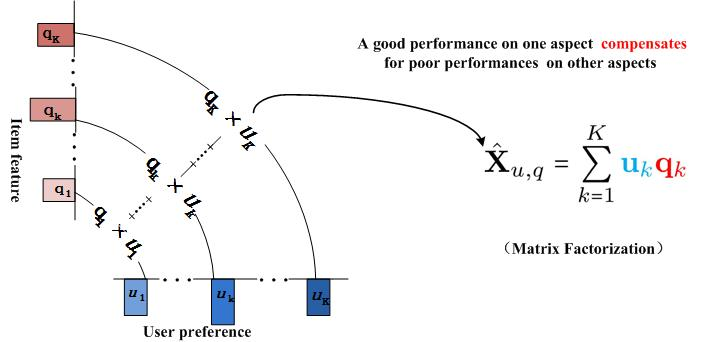
\includegraphics[width=0.55\linewidth]{Compensatory.jpg}
%\end{center}
%\begin{figure}
%\right
%\centering
%\begin{right}
%\begin{center}
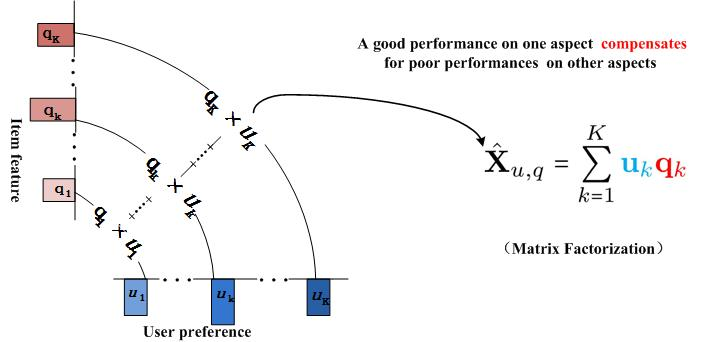
\includegraphics[width=0.95\linewidth]{Compensatory.jpg}
%\end{center}
%\end{right}
%\end{figure}
\item Other Rating Models
%\begin{enumerate}
%\item
%\begin{equation}\label{equ:MF}
% \hat{\mathbf{X}}_{u,q}=\sum_{k=1}^{K} \textcolor{cyan}{\mathbf{u}_k}\textcolor{red}{\mathbf{q}_k}
%\end{equation}

%\begin{itemize}

 AMF@KDD'08: \quad
%\begin{equation*}
$\hat{\Rating}_{u,q}=\sum_{k=1}^{K} \textcolor{cyan}{ (\sum_{\mathbf{p} \in R(u)} \mathbf{p}_k/\sqrt{|R(u)|} )} \textcolor{red}{\mathbf{q}_{k}} $
%\end{equation*}

 LLORMA@JMLR'16:\quad
\begin{equation*}
\hat{\Rating}_{u,q}
= \sum_{t=1}^{S} \sum_{k=1}^K \textcolor{cyan}{\mathbf{u}_{t, k} \frac{K((\mathbf{u}_t,\mathbf{i}_t),(\mathbf{u},\mathbf{q}))}{\sum_{s=1}^{S} K((\mathbf{u}_s,\mathbf{i}_s),(\mathbf{u},\mathbf{q}))}}\textcolor{red}{ \mathbf{q}_{t,k}}
\end{equation*}

%\end{enumerate}
%\item Compensatory Models -- Ranking Models\\
%Thurstone Model:
%\begin{equation*}\label{equ:BPR}
%Pr(p\succ_u q) = \frac{1} {1+\exp[-(\hat{\Rating}_{u,p}-\hat{\Rating}_{u,q})]}
%\end{equation*}


%\end{itemize}
\item Pair-wise Ranking Models
%\begin{itemize}
%\item 

Thurstone Model: BPR@UAI'09,FSBPR@AJSE'18,LCR@WWW'14\\

%\begin{equation*}\label{equ:BPR}
$Pr(p\succ_u q) = \frac{1} {1+\exp[-(\hat{\Rating}_{u,p}+\hat{\Rating}_{u,q})]},\hat{\Rating}_{u,p,q}\textrm{ by MF, AMF, or LLORMA}$\\
%=\sum_{k=1}^{K} \textcolor{cyan}{\mathbf{u}_k}(\textcolor{red}{\mathbf{p}_k-\mathbf{q}_k})
%\end{equation*}

%\item 
Bradley-Terry Model: BT@ICDM'16
\begin{equation*}
Pr(p\succ_u q) = \frac{{\hat{\Rating}_{u,p}}}{{\hat{\Rating}_{u,p}}+ {\hat{\Rating}_{u,q}}} , \quad \textrm{where}\quad  \hat{\mathbf{X}}_{u,q}=\sum_{k=1}^{K} \textcolor{cyan}{\mathbf{u}_k}\textcolor{red}{\mathbf{q}_k}
\end{equation*}


%\end{itemize}
\end{itemize}
}


\headerbox{Rating Prediction}{name=Results1,span=1,column=0,below=Compensatory}{
%\begin{center}
%\begin{itemize}
%\item Comparative rating prediction performances.
%\vspace{-0.14cm}
%\item `Imp.' is the percentage of improvements of non-compensatory versions relative to the original models.
%\item 
\vspace{0.13cm}
$\circ$ Comparative experiments on rating prediction.  \\
$\circ$ Non-compensatory rules universally increase prediction accuracy.\\

\small
%\end{itemize}
\resizebox{0.55\textwidth}{!}{\begin{minipage}{\textwidth}
\begin{tabular}{l l l l l l l}
\toprule
\textbf{Method} & \textbf{AUC} & \textbf{Imp} & \textbf{NDCG} & \textbf{Imp} & \textbf{MRR} & \textbf{Imp} \\
\midrule
Movielens& & $(\%)$ & & $(\%)$ & & $(\%)$\\\hline
MF&	0.6729 &	&	0.6925 &	&	0.8300 &	\\
MF-N&	0.7108 &	5.62&	0.7166 &	3.48&	0.8633 &	4.01\\
AMF&	0.6901 &	&	0.7107 &	&	0.8747 &	\\
AMF-N &	0.7027 	&1.83&	0.7138 &	0.44&	0.8790 	&0.49\\
LLORMA&	0.7265 &	&	0.8734 &	&	0.7015 &	\\
LLORMA-N&	0.7299 &	0.47&	0.8999 &	3.03&	0.7187 &	2.45\\\hline
Filmtrust& & $(\%)$ & & $(\%)$ & & $(\%)$\\\hline
MF&	0.6507 &	&	0.5229 &	&	0.7011 &	\\
MF-N&	0.6710 &	3.12&	0.5241 &	0.23&	0.7071 &	0.86\\
AMF&	0.5971 &	&	0.5137 &	&	0.7411 &	\\
AMF-N&	0.6133 &	2.71&	0.5253 &	2.25&	0.7619 &	2.80\\
LLORMA&	0.6240 &	&	0.8596 &	&	0.7857 &	\\
LLORMA-N&	0.6345 &	1.68&	0.8684 &	1.02&	0.8068 &	2.69\\ \hline
CiaoDVD& & $(\%)$ & & $(\%)$ & & $(\%)$\\\hline
MF&	0.7431 &	&	0.7949 &	&	0.8910 &	\\
MF-N&	0.7903 &	6.34&	0.8127 &	2.25&	0.9154 &	2.74\\
AMF&	0.6489 &	&	0.6612 &	&	0.8741 &	\\
AMF-N&	0.6993 &	7.77&	0.6878 &	4.02&	0.8967 &	2.58\\
LLORMA&	0.6752 &	&	0.7827 &	&	0.8267 &	\\
LLORMA-N&	0.6845 &	1.38&	0.7984 &	2.00&	0.8384 &	1.42\\
\bottomrule
\end{tabular}
\end{minipage}}
\\

%\begin{itemize}
%\item 

%\item
\vspace{0.05cm}
$\circ$ $b_{u,k}$ significantly positive suggests aspect specific cut-off thresholds.\\
$\circ$ Moderate $\theta$ suggests a combination of lexicographic and conjunctive rules.\\

%\end{itemize}
%\centering
%\begin{center}
\resizebox{0.55\textwidth}{!}{\begin{minipage}{\textwidth}
\centering
\begin{tabular}{l l l l l}

\hline
Dataset   &Imp.($\%$)& $\sigma(\mathbf{b}_{u})$& $\theta$ \\\hline
Movielens & 5.37 & $0.0095\pm0.0024$ & $0.608\pm 0.105$  \\
FilmTrust & 2.21 & $0.0095\pm0.0023$ & $0.667\pm 0.016$\\
CiaoDVD & 28.97 & $0.0093\pm0.0022$  &$0.773\pm 0.051$\\\hline

%Statistics of Datasets with ratings& & & & \\\hline
%Dataset & \#users & \#items & \#ratings & \#pairs \\\hline
%Movielens &942 &1,650 &80,000 & 1,072,237 \\\hline
%Filmtrust &1,235 &2,062 &35,497 &623,516 \\\hline
%CiaoDVD &2,665 &14,280 &72,665 &2,478,836 \\\hline

\end{tabular}
\end{minipage}}
%\end{center}
%\begin{table}[htp]
%\caption{Statistics of Datasets with ratings}
%\small
%\centering
%\scalebox{0.9}{
%\begin{tabular}{|c|c|c|c|c|}
%\hline
%Dataset & \#users & \#items & \#ratings & \#pairs \\\hline
%Movielens &942 &1,650 &80,000 & 1,072,237 \\\hline
%Filmtrust &1,235 &2,062 &35,497 &623,516 \\\hline
%CiaoDVD &2,665 &14,280 &72,665 &2,478,836 \\\hline
%\end{tabular}}
%\label{tab:datasets}
%\end{table}

%\end{center}
%\begin{center}
%\end{center}
}

\headerbox{Explicit Feedback}{name=Results2,span=1,column=1,below=Compensatory}{

$\circ$  Comparative results for ranking reconstruction, pairwise ranking observed from explicit feedback, i.e. a higher rating is considered to be superior than a lower rating. \\
$\circ$  Non-compensatory rules generally improve ranking performance.\\


\resizebox{0.55\textwidth}{!}{\begin{minipage}{\textwidth}
\begin{tabular}{l l l l l l l}
\toprule
\textbf{Method} & \textbf{AUC} & \textbf{Imp} & \textbf{NDCG} & \textbf{Imp} & \textbf{MRR} & \textbf{Imp}\\
\midrule
Movielens& & $(\%)$ & & $(\%)$ & & $(\%)$\\\hline
BT&0.6453 & & 0.5329 & & 0.8227 & \\
BT-N& 0.8511 & 31.89& 0.5795 & 8.74& 0.9256 & 12.51\\
BPR	&0.7976	&&	0.5674	&&	0.8988	&\\
BPR-N	&0.8361	&4.82&	0.5761&	1.53&0.9180	&2.14\\
FSBPR	&0.5048 	&&	0.5011 	&&	0.7524 	&\\
FSBPR-N&	0.8272 &63.86&	0.5740 &	14.56&	0.9136 &	21.42\\
LCR&	0.7191&&		0.8555&&		0.9461	&\\
LCR-N&	0.7360	&2.35&	0.8605&	0.58&	0.9515&	0.57\\
\hline
FIlmtrust& & $(\%)$ & & $(\%)$ & & $(\%)$\\\hline
BT& 0.5405 & & 0.5092 & & 0.7702 & \\
BT-N & 0.6969 & 28.94& 0.5446 & 6.95& 0.8485 & 10.15\\
BPR&	0.6412	&&	0.5319	&&	0.8206&\\	
BPR-N	&0.6729	&4.94&	0.5391	&1.35&	0.8364&	1.93\\
FSBPR	&0.4857 	&&	0.4968 &&		0.7428 	&\\
FSBPR-N	&0.6717 &	38.29&	0.5388 &	8.47&	0.8358 &	12.52\\
LCR	&0.5977&&		0.9034	&&	0.7511	&\\
LCR-N&	0.6144&	2.79&	0.9063	&0.32&	0.7635	&1.65\\
\hline
CiaoDVD& & $(\%)$ & & $(\%)$ & & $(\%)$\\\hline
BT& 0.6063 & & 0.5240 & & 0.8031 & \\
BT-N& 0.9334 & 53.95& 0.5981 & 14.1& 0.9666 & 20.36\\
BPR	&0.6344	&&	0.5304&&		0.8172	&\\
BPR-N	&0.8987	&41.66&0.5902&	11.28&	0.9493&	16.17\\
FSBPR	&0.7537 	&&	0.5574 	&&	0.8769 	&\\
FSBPR-N&	0.8992 &	19.30&	0.5903 &	5.91&	0.9496 &	8.30\\
LCR&	0.6260	&&	0.9408	&&	0.7889	&\\
LCR-N	&0.6349&	1.42&	0.9451&	0.46&	0.7988&	1.25\\
\bottomrule
\end{tabular}
\end{minipage}}
}

%----------------------------------------------------------------------------------------
%	MEASUREMENT SETUP
%----------------------------------------------------------------------------------------
%\headerbox{Experiment Results2 }{name=ExperimentResults,span=2,column=1,below=Results1}{
%%\begin{center}
%
%%\end{center}
%}

\headerbox{Non-Compensatory Models}{name=NonCompensatory,column=2,span=2,below=Abstract}{
\begin{itemize}
\item Non-Compensatory Decision Rule
\begin{center}
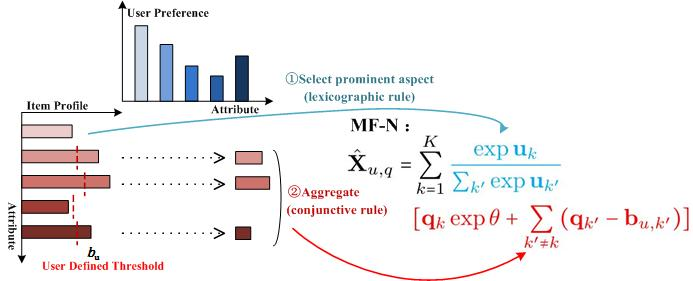
\includegraphics[width=0.90\textwidth]{NonCompensatory.jpg}
\end{center}
\item Other Non-Compensatory Rating Models
%\begin{itemize}
%\item MF-N:
%\begin{equation*}\label{equ:MF-N}
%\begin{aligned}
% \hat{\mathbf{X}}_{u,q} = & \sum_{k=1}^{K}\textcolor{cyan}{\frac{\exp \mathbf{u}_k}{\sum_{k'} \exp \mathbf{u}_{k'}}} \\\nonumber
% & \textcolor{red}{[ \mathbf{q}_k  \exp\theta  + \sum_{k'\neq k} (\mathbf{q}_{k'}-\mathbf{b}_{u,k'}) ]}
% \end{aligned}
%\end{equation*}

%\item 
AMF-N:
 %\begin{eqnarray*}\label{equ:AMF-N}
 $\hat{\mathbf{X}}_{u,q} = \sum_{k=1}^{K} \textcolor{cyan}{\frac{\exp (\sum_{\mathbf{p} \in R(u)} \mathbf{p}_k )}{\sum_{k'} \exp  (\sum_{p \in R(u)} \mathbf{p}_{k'} ) } } %\\\nonumber
 \textcolor{red}{[  \mathbf{q}_k \exp\theta + \sum_{k'\neq k} (\mathbf{q}_{k'}-\mathbf{b}_{u,k'})]}$
%\end{eqnarray*}
%\item 
LLORMA-N:
\begin{eqnarray*}\label{equ:LLORMA-N}
\hat{\Rating}_{u,q} = & \sum_{t=1}^{S} \sum_k  \textcolor{cyan}{\frac{\exp \mathbf{u}_k}{\sum_{k'} \exp \mathbf{u}_{k'}}  \frac{K((\mathbf{u}_t,\mathbf{i}_t),(\mathbf{u},\mathbf{q}))}{\sum_{s=1}^{S} K((\mathbf{u}_s,\mathbf{i}_s),(\mathbf{u},\mathbf{q}))}} \\\nonumber
&\textcolor{red}{ [ \mathbf{q}_{t,k} \exp\theta  + \sum_{k'\neq k} (\mathbf{q}_{t,k'}-\mathbf{b}_{u,k'})]}
\end{eqnarray*}
%\end{itemize}

\item Non-Compensatory Pair-wise Ranking Models\\
%\begin{itemize}
%\item 
Thurstone Model - N:\\

%\begin{eqnarray*}\label{equ:AMF-N}
$\hat{\mathbf{X}}_{u,p,q} = \sum_{k=1}^{K} \textcolor{cyan}{\frac{\exp (\mathbf{u}_k )}{\sum_{k'} \exp (\mathbf{u}_{k'} ) } } %\\\nonumber
 \textcolor{red}{[\exp\theta  (\mathbf{p}_k-\mathbf{q}_k ) + \sum_{k'\neq k} (\mathbf{p}_{k'}-\mathbf{q}_{u,k'})]}$\\
 
%\end{eqnarray*}
%\item 
Bradley Terry Model - N:
\begin{equation*}
Pr(p\succ_u q)  =  \sum_{k=1}^{K} \textcolor{cyan}{\mathbf{u}_k} \textcolor{red}{[ {\frac{\mathbf{p}_k}{\mathbf{p}_k+\theta \mathbf{q}_k}} \prod_{k'\neq k}{ \frac{\theta \mathbf{p}_{k'}}{\mathbf{q}_{k'}+\theta \mathbf{p}_{k'}}}]}
\end{equation*}
%\end{itemize}
\end{itemize}
}

\headerbox{Implicit Feedback}{name=Results3,column=2,below=NonCompensatory,span=2}{
%\begin{center}

\vspace{0.25cm}
$\circ$  Comparative results for ranking reconstruction, pairwise ranking observed from implicit feedback which is graded, i.e. a purchase is considered superior than a click, more details refer to our paper.\\

$\circ$  Non-compensatory rules generally improve ranking performance on implicit feedback.\\


\resizebox{0.58\textwidth}{!}{\begin{minipage}{\textwidth}
\begin{tabular}{l l l l l l l l l l l l}
\toprule
 & \textbf{Method} & \textbf{AUC} & \textbf{Imp.$(\%)$} & \textbf{NDCG} & \textbf{Imp.$(\%)$} & \textbf{MRR} & \textbf{Imp.$(\%)$}  & \textbf{MAP} & \textbf{Imp.$(\%)$}  & \textbf{Prec} & \textbf{Imp.$(\%)$}\\
\midrule
 Tmall-single\\\hline
& BT	&0.5304 	&	&0.2804 	&	&0.4870 	&	&0.4327 	&	&0.2778 &\\
& BT-N	&0.5400 	&1.82	&0.2840 	&1.28	&0.4948 	&1.61	&0.4386 	&1.34	&0.2801 & 0.84\\
& BPR&	0.5181	&&	0.2794	&&	0.4854	&&	0.4297	&&	0.2767&\\	
& BPR-N	&0.5349&	3.24&	0.2848	&1.92&	0.4960	&2.18&	0.4401&	2.41&	0.2806	&1.41\\
&FSBPR	&0.5265 	&&	0.2824 	&&	0.4913 	&&	0.4350 	&&	0.2794 	&\\
&FSBPR-N	&0.5389& 	2.35&	0.2863 	&1.39&	0.4988 &	1.53&	0.4432 &	1.90&	0.2818 &	0.87\\
&LCR&	0.5200 	&&	0.8190 	&&	0.4277 	&&	0.3568 	&&	0.2534 	&\\
&LCR-N&	0.5290 &	1.73&	0.8213 &	0.28&	0.4360 	&1.94&	0.3648 	&2.24&	0.2586 &	2.05\\
\hline
Tmall-hybrid\\\hline
&BT	&0.5867 	&	&0.3015 	&	&0.5373 	&	&0.4929 	&	&0.2904 & \\
&BT-N	&0.6568 	&11.94	&0.3279 	&8.75	&0.5990 	&11.48	&0.5527 	&12.13	&0.3036 &4.53 \\
&BPR	&0.6183&	&	0.3183&&		0.5792	&&	0.5318&&		0.2973&\\	
&BPR-N	&0.6460	&4.48&	0.3276&	2.92&0.5990	&3.41&	0.5524&	3.87&	0.3030	&1.94\\
&FSBPR	&0.6334 	&&	0.3246 	&&	0.5916 &&		0.5442 	&&	0.3026 	&\\
&FSBPR-N&	0.6544 &	3.31&	0.3309 &	1.94&	0.6062 &	2.48&	0.5603 &	2.95&	0.3047 &	0.69\\
&LCR	&0.5398 	&&	0.6644 	&&	0.4519 	&&	0.3745 	&&	0.2597 	&\\
&LCR-N&	0.5649 &	4.65&	0.6790 &	2.20&	0.4809 &	6.42&	0.3988 &	6.49&	0.2720 &	4.74\\
\hline
Yoochoose\\\hline
&BT	&0.6027 	&	&0.4734 	&	&0.7151 	&	&0.6361 	&	&0.4560 & \\
&BT-N	&0.7000 	&16.15	&0.5160 	&8.99	&0.7869 	&10.04	&0.7084 	&11.37	&0.4785  &4.92\\
&YBPR&	0.6700	&&	0.5065	&&	0.7713&&		0.6895	&&	0.4737&\\	
&BPR-N	&0.6920	&3.28&	0.5131	&1.31&	0.7812&	1.29&	0.7027	&1.91&	0.4771	&0.74\\
&FSBPR	&0.3272 	&&	0.3658 	&&	0.5062 	&&	0.4599 	&&	0.4006 	&\\
&FSBPR-N	&0.6198 &	89.45&	0.4822 &	31.83&	0.7169& 	41.62&	0.6448 &	40.22&	0.4650 &	16.08\\
&LCR	&0.5842 	&&	0.9725 	&&	0.8009 &&		0.7934 	&&	0.7677 	&\\
&LCR-N&	0.6315 &	8.10&	0.9754 &	0.30&	0.8231 &	2.77&	0.8161 &	2.86&	0.7881 &	2.66	\\

\bottomrule
\end{tabular}
\end{minipage}}
%\end{center}
}


%----------------------------------------------------------------------------------------
%	CONCLUSION
%----------------------------------------------------------------------------------------
\headerbox{Conclusion}{name=conclusion,column=0,below=Results1,span=2}{
\begin{itemize}
\item Existing recommendation models are based on compensatory decision rules. However,consumers adopt non-compensatory rules more often. % in real life
\vspace{-0.09cm}
\item We propose a non-compensatory framework which can be easily embedded in latent factor models. We experimentally show that it universally improves recommendation performances of different existing models.
\vspace{-0.09cm}
\item This contribution sheds insight to developing explainable shallow models.
\end{itemize}
}

\headerbox{Acknowledgments}{name=Acknowledgments,column=2,below=Results3,span=2}{
\vspace{0.2cm}
Chen Lin is supported by Natural Science Foundation of China under grant No.61472335. Yanghua Xiao is supported by NSFC (No.61732004, No.61472085, No.U1509213, No.U1636207), National Key R\&D Program of China (No.2017YFC0803700, No.2017YFC1201200), Shanghai Municipal Science and Technology project (No.16511102102, No.16JC1420401), Shanghai STCSMs R\&D Program (No.16JC1420400).
\vspace{0.1cm}
}

\end{poster}
\end{document}
